% INNAN DU COMMITAR!
% Uppdatera datum
% Uppdatera version
%-----
% Document name



\documentclass[10pt,a4paper]{article}
\usepackage[utf8]{inputenc}
\usepackage[english]{babel}
\usepackage{amsmath}
\usepackage{amsfonts}
\usepackage{amssymb}
\usepackage{graphicx}
\usepackage{geometry}

\title{PostCardBuddy}
\author{Team C}

\begin{document}
\begin{titlepage}
\newgeometry{left=2cm,top=1cm,right=2cm}
\newcommand{\HRule}{\rule{\linewidth}{0.5mm}}


\begin{flushright}
November 20, 2015 v0.05\\[3cm]
\end{flushright}


\centering
\textsc{\LARGE Team C}\\[0.5cm]

\HRule \\[0.4cm]
{ \huge \bfseries PostCardBuddy}\\[0.3cm]
{\Large \bfseries Project Experiences}\\[0.4cm] % Title of your document
\HRule \\[1.5cm]

\vfill
\begin{flushleft}
%Authors, write on separate lines
\textit{Authors of this document:}\\
Emma Albertz\\
Caroline Brandberg\\
Linnéa Claesson\\
Billy Johansson\\
Johan Ju\\
Jacob Mejvik\\
Carl Rynegardh
\end{flushleft}

\end{titlepage}
\pagenumbering{gobble}



%\begin{center}
%\textit{\large Version History}
%
%    \begin{tabular}{ | l | l | l | p{5cm} |}
%    \hline
%    \textbf{Version} & \textbf{Date} & \textbf{Responsible} & \textbf{Description} \\ \hline
%    1.0 & 2015-10-14 & EA, LC & Baseline\\ \hline
%    \end{tabular}
%\end{center}



\setcounter{tocdepth}{2}
\tableofcontents
\newpage
\pagenumbering{arabic}

%---------------------------------------------------------------%
% A description of our requirements engineering work, including experiences and reflections in relation to learning objectives.
% The Project Experiences should not include course evaluation issues, but focus on your own work and learning outcome.
%---------------------------------------------------------------%

%-------------------------------------------------------------------%
%-------------- Background -----------------------------------------%
%-------------------------------------------------------------------%
\section{Background}
During the first week, and the work for release one, we have worked to figure out who our stakeholders are and what they would like to see from our system. We have used a lot of different elicitation techniques and tried to keep requirements at a fairly high level, goal- or domain-level. Finding requirements through different elicitation techniques have been the highest ranked priority for release one.


%-------------------------------------------------------------------%
%--------------- Methods and Techniques ----------------------------%
%-------------------------------------------------------------------%
% Description of the chosen methods/techniques for elicitation, specification, validation, and prioritization.
% Motivation for why you chose the used methods/techniques.
\section{Methods and Techniques}




% 3D) apply more than one elicitation technique in a relevant way.
\subsection{Elicitation}
We techniques we have used have been inspired by "Software Requirements Style and Techniques" chapter 8, written by Soren Lauesen. The figure 8.2, page 338, has been of great help in choosing appropriate elicitation techniques.
For release one we used the techniques: Brainstorming, Questionnaires, Prototypes, Focus groups, Document studies, ask suppliers and stakeholder analysis. !!!!! <-  THIS , Har vi gjort allt detta?
/newline
Brainstorming: To come up with different functions we at first used brainstorming writing down the functions we could come up with. During the brainstorming session we also thought about, and extended, the specification and function given to us after the first week.
\newline
Questionnaire: The questionnaire contained functions that we came up with during the brainstorming session. Persons answering where asked to grade functions with grade 0-5, where zero stood for not interesting and five for very interesting. We also added a field for age to see if we could make out a difference in the interest of different functions between ages, stakeholders.
\newline
Prototypes: As we are time constrained, we decided to already create prototypes. Three of us made our own prototypes. As we are early in making requirements it was only about coming up with ideas for the graphical design of the app. In order not to affect the ideas of each other we designed them in isolation. 
Prototypes is a suitable technique for our product because of that we are specifying an application for end users. It helps the elicitation process by having uses say "Can I do that here" when they test the prototype. 
\newline
Document studies: As there already is an app on the market for sending physical postcards having a look at its featured seemed like a good idea. This was first done after brainstorming and thinking of functions of our own so that we would not kill our own creativity. Also, creating the same app over again does not seem like a good idea, referring to business goal such as that it should be able to create revenue. By studying the already existing app we hope to find ways to make it better. We have not put down a lot of effort in this yet. This will probably be done more thoroughly for release 2.
\newline
Focus group: Should be added.
\newline
Stakeholder analysis: Should be added.



% 4B) use at least four different specification techniques adequately tailored to the context.
\subsection{Specification}
Context diagram: A context diagram will be used because of its strengths to be easy to use at validation and verification. The diagram gives a good over-view of the system, both for the use of the client but also for the developers. 
% 3F) to assess the quality of requirements and find relevant problems of several different types.
% 3G) apply more than one validation technique.
% 4G) adapt the validation to the context and provide rationale for the chosen validation techniques.
\subsection{Validation}
Prototypes: The prototype gives our customer a unique opportunity to validate how our product match their expectations. We are trying to contentiously adapt the prototype to our customers needs and new features so that it becomes a good reflection on where the project is going.

% 3I) use more than one prioritization technique in a relevant way.
\subsection{Prioritization}

%--------------------------------------------------------------------%
%--------------- Reflections ----------------------------------------%
%--------------------------------------------------------------------%
% Reflection on the usage of these methods/techniques in terms of what was successful and what was challenging. Example questions for reflection: What have you learned in relation to the learning objectives in this course program? What would you have done differently if you would do this project again as a "real" project, based on what you know now? What have you learned in relation to the learning objectives?


% Osäker om detta är rätt placering: 5B) provide motivated estimations of target quality levels using well-defined scales.
% 4F) to find, prioritize and discuss requirements quality problems of different types, while reaching 	beyond form issues.
% 5D) reason about the relation between requirements quality problems and risks, both from a customer and developer viewpoint.
\section{Reflections}

% 3E) reflect on elicitation experiences.
% 4E) reason about the need for further elicitation in relation to specification quality.
% 5C) go beyond initial stakeholders and given frames, while challenging the domain boundaries and eliciting creative ideas and deep domain knowledge in real-world contexts.
\subsection{Elicitation}
Prototypes: We found an easy to use program for constructing prototypes that have worked very well for us. When we made many individual prototypes we discoverer that it also worked as practical brainstorming where we found features in the prototypes.
\newline
Questionnaire: Figure~\ref{fig:questionnaire} present the result of the questionnaire, which 38 persons have answered. To get answers from that amount of people was no problem, but it still gave a start of what the users were interested in. The result of this is that the functionality "Share postcard on social media" was not important and "Suggestion for GPS-based images" was appreciated. This will be considered under release 2. The result also shows that the desired functionality didn't change that much depending on the age.
\newline
Document studies: The already existing app is easy to use and slim. It does not contain a lot of functions but there are enough. Most of the basic functions we have been thinking of are already implemented. However, there are definitely some functionalities that could be of use that is not implemented. Also, the library of images is not very big and GPS based images depending on your localization only work in Sweden and Denmark.

\begin{figure}[h!]
\centering
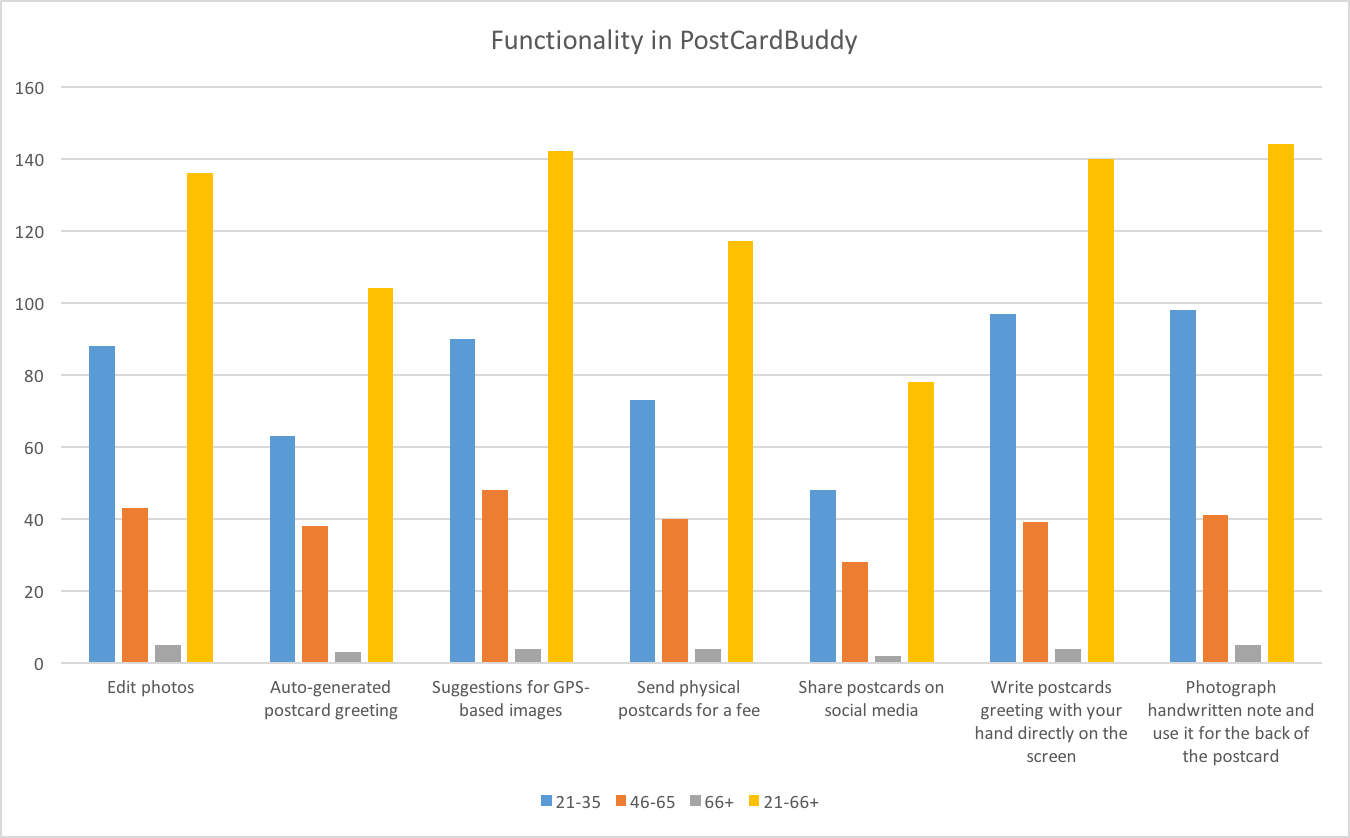
\includegraphics[width=1.0\textwidth]{questionnaire.png}
\caption{Result of the questionnaire on the desired functionality in PostCardBuddy}
\label{fig:questionnaire}
\end{figure}
% Ska vi �ven ha en figur som presenterar hur m�nga 0,1,..5 varje funktion fick???


% 3C) reflect on specification experiences and reason about choices of specification methods in relation to different contexts.
% 5A) combine specification techniques in an explicitly motivated trade off between qualities and costs, where a high degree of specification completeness is achieved for a carefully selected subset of requirements.
\subsection{Specification}
Context Diagram: The first context diagram created is presented in PMv2. The first diagram is very limited and contains too little information to understand the system. The updated diagram is presented in release 1 of the report System Requirements. The biggest problem creating a context diagram is that it should be big enough to present important details, but small enough to be able to get a over-view of the system. Therefore it is very important to think through which components it should contain, and which should be left out. This difference is often personal, which we noticed during the creation of release 1, which led to some discussion. The most time of the discussion were spend talking about if the back-end should be presented and how the functionality that is used within the mobile should be presented. 

% 3H) reflect on validation experiences.
% 5E) utilize links among different types of specifications in validation efforts to find and address potentially harmful inconsistencies.
\subsection{Validation}

% 3J) reflect on prioritization experiences.
\subsection{Prioritization}

%--------------------------------------------------------------------%
%------------ Personal Statements -----------------------------------%
%--------------------------------------------------------------------%
% A personal statement by each team member that briefly explains each individual's contributions to the project results.
\section{Personal Statements}



\end{document}

